
\documentclass[10 pt,usenames,dvipsnames, oneside]{article}
\usepackage{../../modelo-fracoes}
\graphicspath{{../../../Figuras/licao03/}}


\begin{document}

\begin{center}
  \begin{minipage}[l]{3cm}

\includegraphics[width=2cm]{../../../Figuras/logo}       
\end{minipage}\hfill
\begin{minipage}[r]{.8\textwidth}
 {\Large \scshape Atividade: O percurso da tartaruga}  
\end{minipage}
\end{center}
\vspace{.2cm}

\ifdefined\prof
%Caixa do Para o Professor
\begin{goals}
%Objetivos específicos
\begin{enumerate}
\item Representar na reta numérica uma fração dada.
\item Estabelecer a comparação entre frações a partir da representação na reta numérica.
\end{enumerate}

\tcblower

%Orientações e sugestões
\begin{itemize}
\item Para responder à questão, não há necessidade de uma informação precisa da posição da tartaruga. A representação das frações indicadas para serem comparadas com a localização da tartaruga não geram dúvida sobre estarem antes ou após a posição da tartaruga, apesar de essa posição não corresponder claramente a um único ponto na reta numérica.
\item É solicitado que os alunos escrevam a justificativa para a avaliação de cada item. Essa decisão tem como objetivo fazer com que o aluno vá além da argumentação oral, mas que consiga organizar as ideias para se expressar por escrito.
\item Observe que o caminho está repartido em 24 partes iguais, ainda que não haja frações sugeridas. A ideia é que cada aluno possa, sozinho, decidir sobre os pontos correspondentes à metade, a quartos, a oitavos e a terços. Discuta essas marcações com os alunos.
\item Cabe observar que cada item pode ser resolvido de forma independente. Por exemplo, para decidir se a posição da tartaruga corresponde a mais do que       $\frac{3}{8}$       do percurso total, o aluno deve identificar oitavos na reta numérica. Já para decidir se a tartaruga já percorreu menos do que       $\frac{2}{3}$       do percurso total, deve identificar terços. Assim, não há necessidade de comparar oitavos com terços.
\item O item h) envolve termo comparativo diferente de ``maior do que'' e ``menor do que''. A expressão ``pelo menos'' oferece outra forma de avaliar a comparação. Explore essa diferença, certificando-se de que os alunos compreenderam.
\item Os itens i) e j) exigem que os estudantes façam uma ``leitura'' da reta numérica ainda não experimentada. Precisam observar, em relação ao percurso total (que é a unidade), a fração correspondente ao que falta ser percorrido.
\item Há vários raciocínios possíveis para responder aos diversos itens desta atividade. Incentive seus alunos a explicarem como raciocinaram, ressaltando, sempre que possível, as diferentes soluções.
\end{itemize}
\end{goals}

\bigskip
\begin{center}
{\large \scshape Atividade}
\end{center}
\fi

A imagem a seguir ilustra uma tartaruga percorrendo um caminho em linha reta, do ponto de partida ao de chegada. Observe a posição da tartaruga na imagem e avalie se as afirmações a seguir estão corretas ou não. Em cada item, explique a sua avaliação por escrito.

\begin{figure}[H]
\centering

\noindent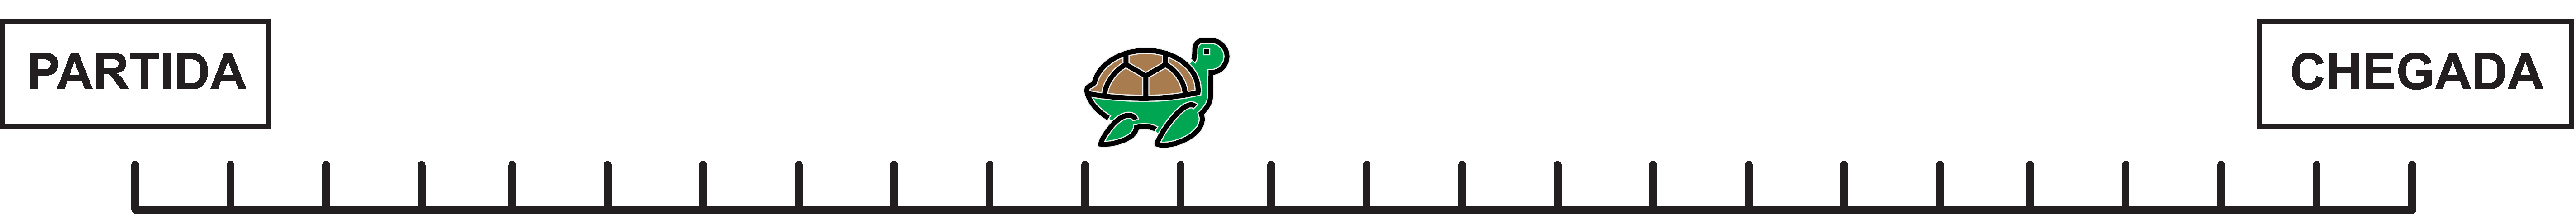
\includegraphics[width=390pt, keepaspectratio]{ativ9_fig01b.png}
\end{figure}

\begin{enumerate} %s
\item     A tartaruga percorreu mais do que a metade do percurso total.
\item     A tartaruga percorreu mais do que     $\frac{3}{4}$     do percurso total.
\item     A tartaruga percorreu mais do que     $\frac{3}{8}$     do percurso total.
\item     A tartaruga percorreu menos do que     $\frac{3}{4}$     do percurso total.
\item     A tartaruga percorreu menos do que     $\frac{2}{8}$     do percurso total.
\item     A tartaruga percorreu menos do que     $\frac{2}{3}$     do percurso total.
\item     A tartaruga percorreu     $\frac{3}{4}$     do percurso total.
\item     A tartaruga percorreu pelo menos     $\frac{5}{8}$     do percurso total.
\item     Para alcançar a chegada, a tartaruga precisa percorrer mais do que a metade do percurso total.
\item     Para alcançar a chegada, a tartaruga precisa percorrer menos do que     $\frac{2}{3}$     do percurso total.
\end{enumerate} %s

\ifdefined\prof
\begin{solucao}

\begin{enumerate}
\item Não está correta. Marcando-se o ponto correspondente à metade do percurso, é fácil verificar que a tartaruga ainda não alcançou esse ponto. 
\begin{center} 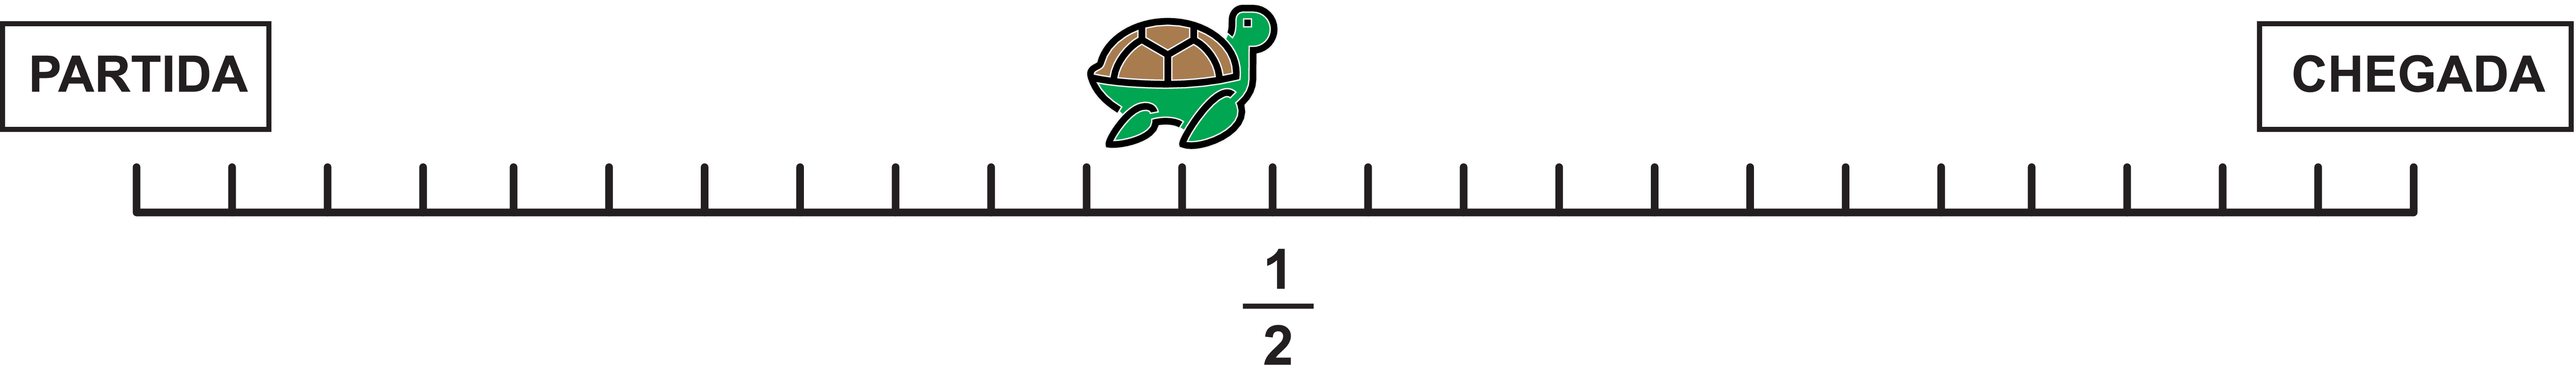
\includegraphics[width=390pt,keepaspectratio]{ativ9_resp_a}
\end{center}
\item  Não está correta. Dividindo-se o percurso em quartos, como ilustra a figura a seguir, fica claro que o ponto correspondente a     $\frac{3}{4}$     do percurso está adiante da localização da tartaruga.
\begin{center}
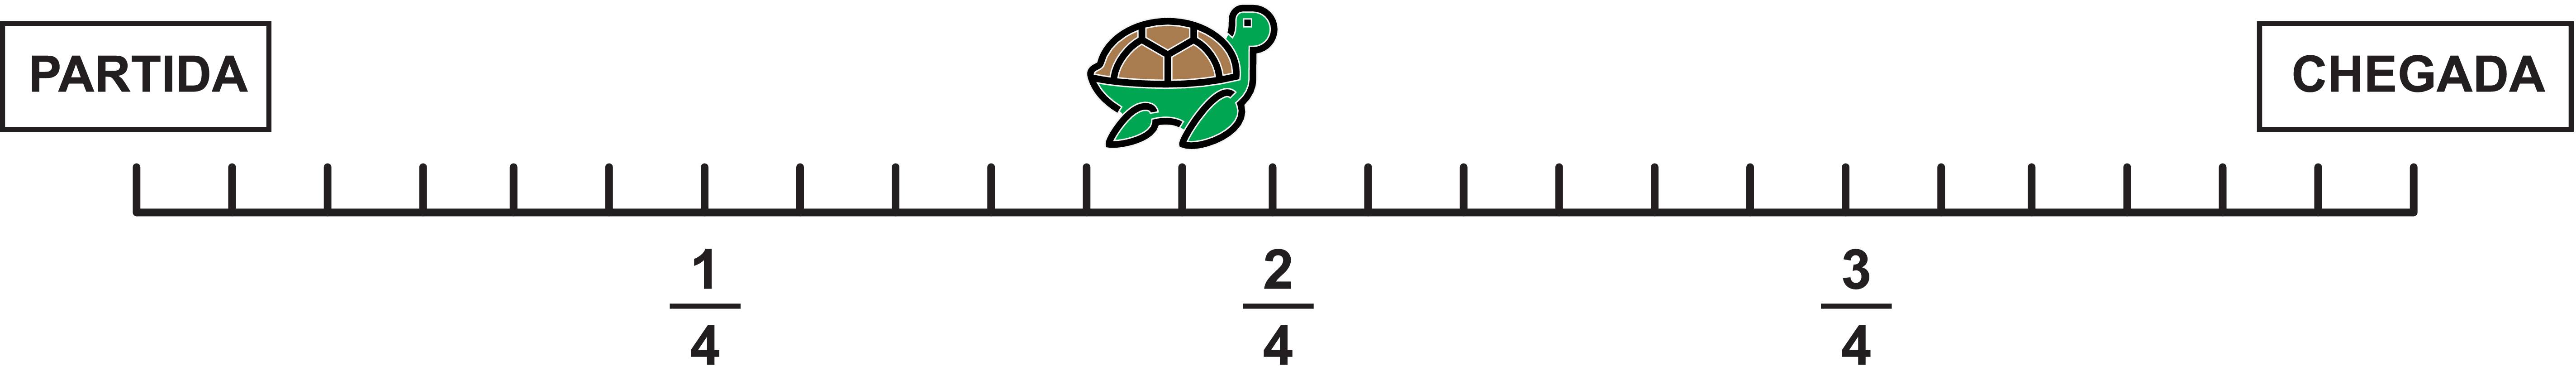
\includegraphics[width=390pt, keepaspectratio]{ativ9_resp_b}
\end{center}
\item     Está correta. Dividindo-se o percurso em oitavos, como ilustra a figura a seguir, fica claro que o ponto correspondente a     $\frac{3}{8}$     do percurso está antes da localização da tartaruga.
\begin{center} 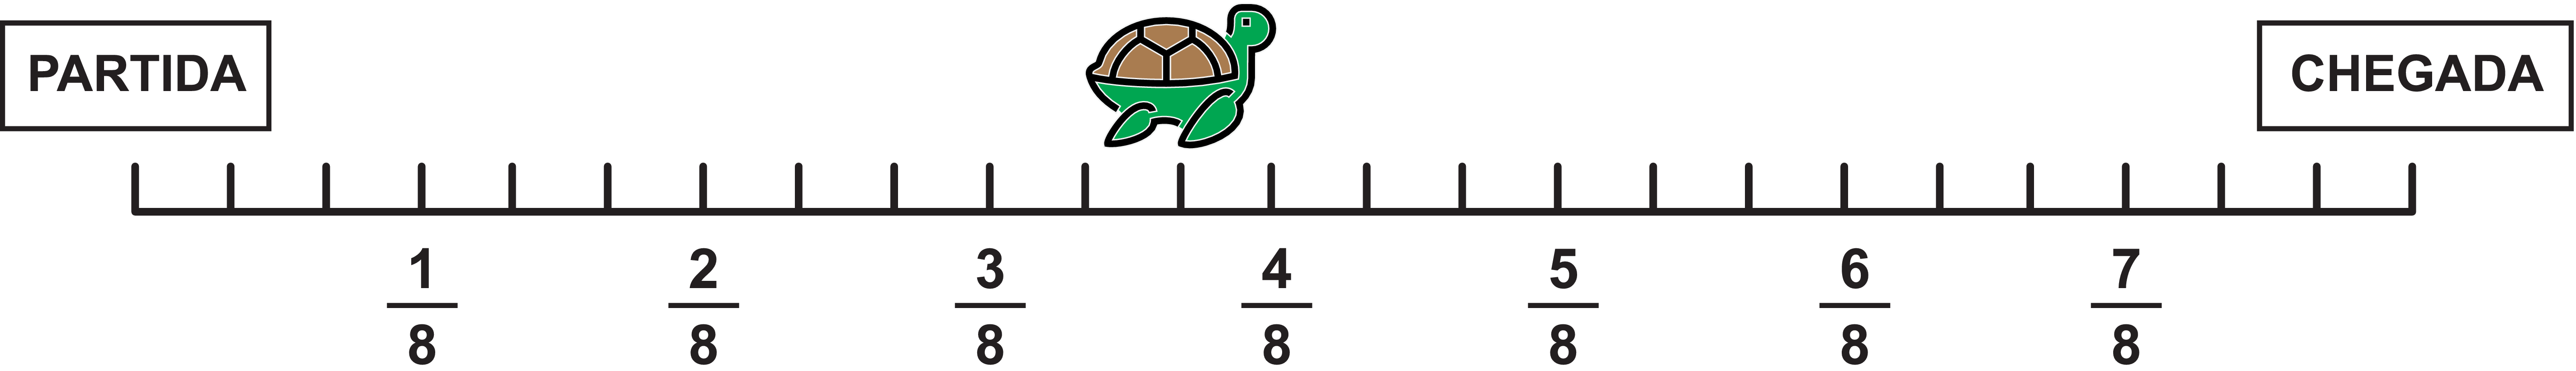
\includegraphics[width=390pt,keepaspectratio]{ativ9_resp_c} 
\end{center}
\item     Está correta. Dividindo-se o percurso em quartos, como ilustra a figura a seguir, verifica-se que a localização da tartaruga é anterior ao ponto correspondente a     $\frac{3}{4}$     do percurso.
\clearpage
\begin{center} 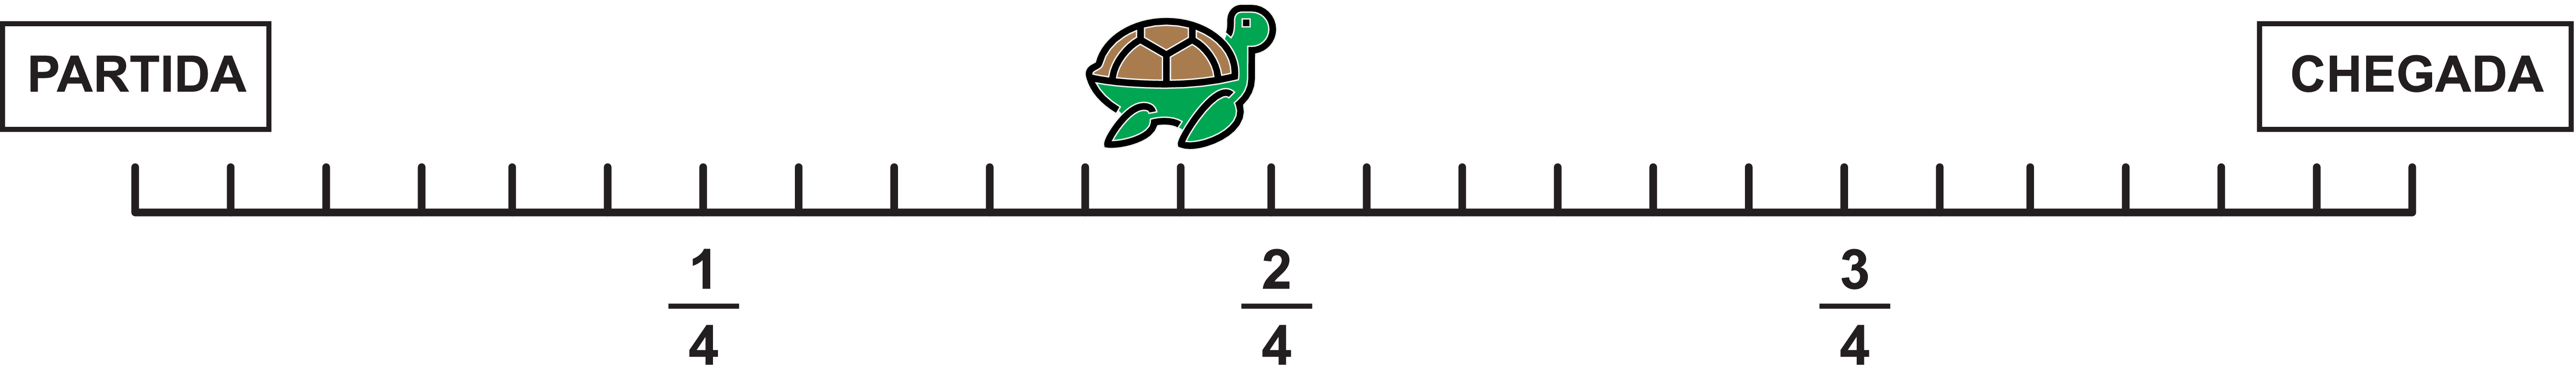
\includegraphics[width=390pt, keepaspectratio]{ativ9_resp_d}
\end{center}

\item     Não está correta. Dividindo-se o percurso em oitavos, como ilustra a figura a seguir, fica claro que o ponto correspondente a     $\frac{2}{8}$     do percurso está antes da localização da tartaruga. 
\begin{center}
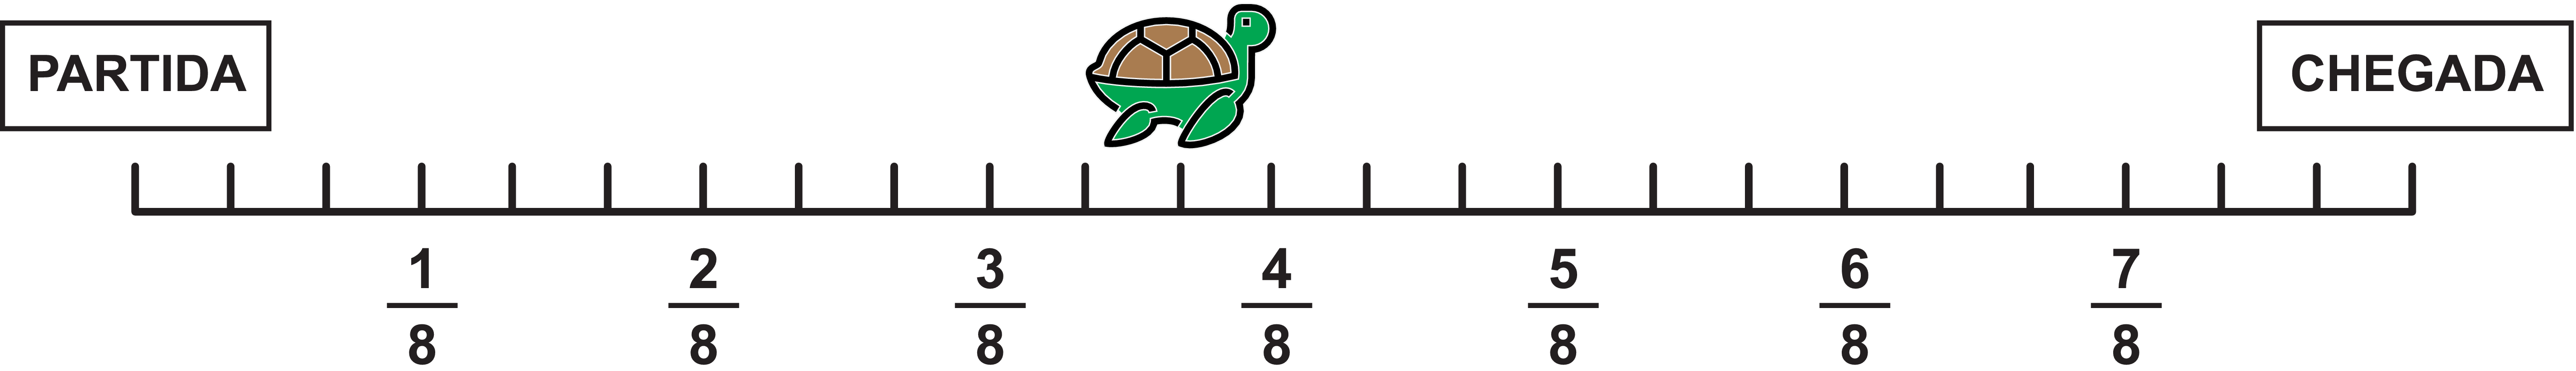
\includegraphics[width=390pt, keepaspectratio]{ativ9_resp_e}
\end{center}

\item     Está correta. Dividindo-se o percurso em terços, fica claro que o ponto correspondente a     $\frac{2}{3}$     do percurso está adiante da localização da tartaruga.

\begin{center} 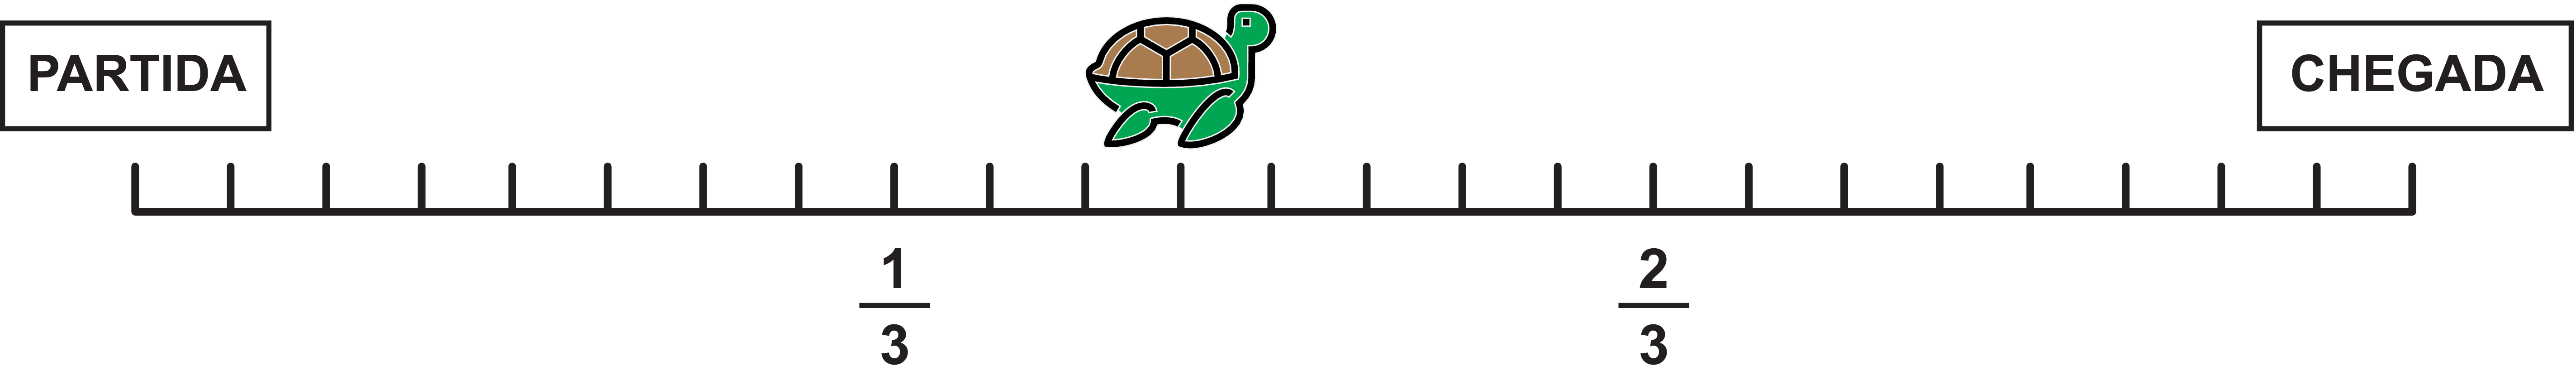
\includegraphics[width=390pt, keepaspectratio]{ativ9_resp_f}
\end{center}


\item     Não está correta. Dividindo-se o percurso em quartos, como ilustra a figura a seguir, fica claro que o ponto correspondente a     $\frac{3}{4}$     do percurso está adiante da localização da tartaruga.

\begin{center} 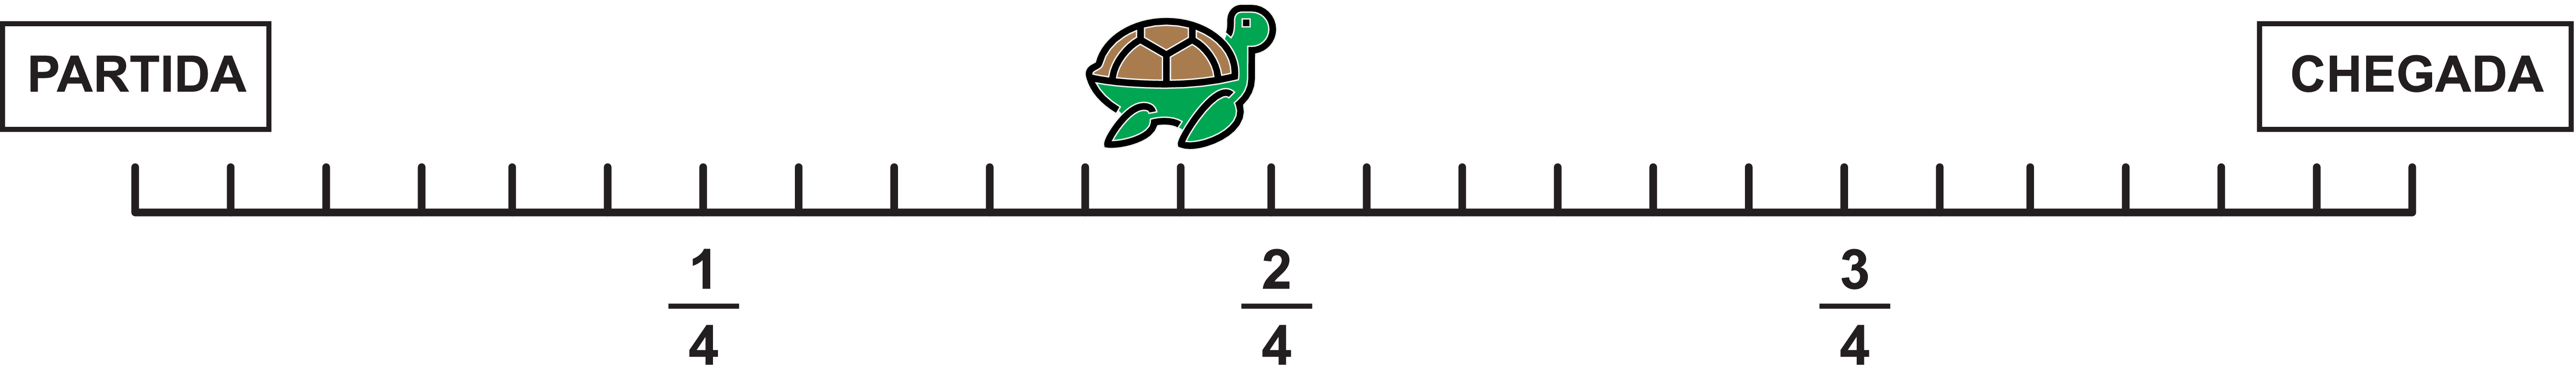
\includegraphics[width=390pt, keepaspectratio]{ativ9_resp_g}
\end{center}

\item     Não está correta. Dividindo-se o percurso em oitavos, fica claro que o ponto correspondente a     $\frac{5}{8}$     do percurso está adiante da localização da tartaruga.

\begin{center}
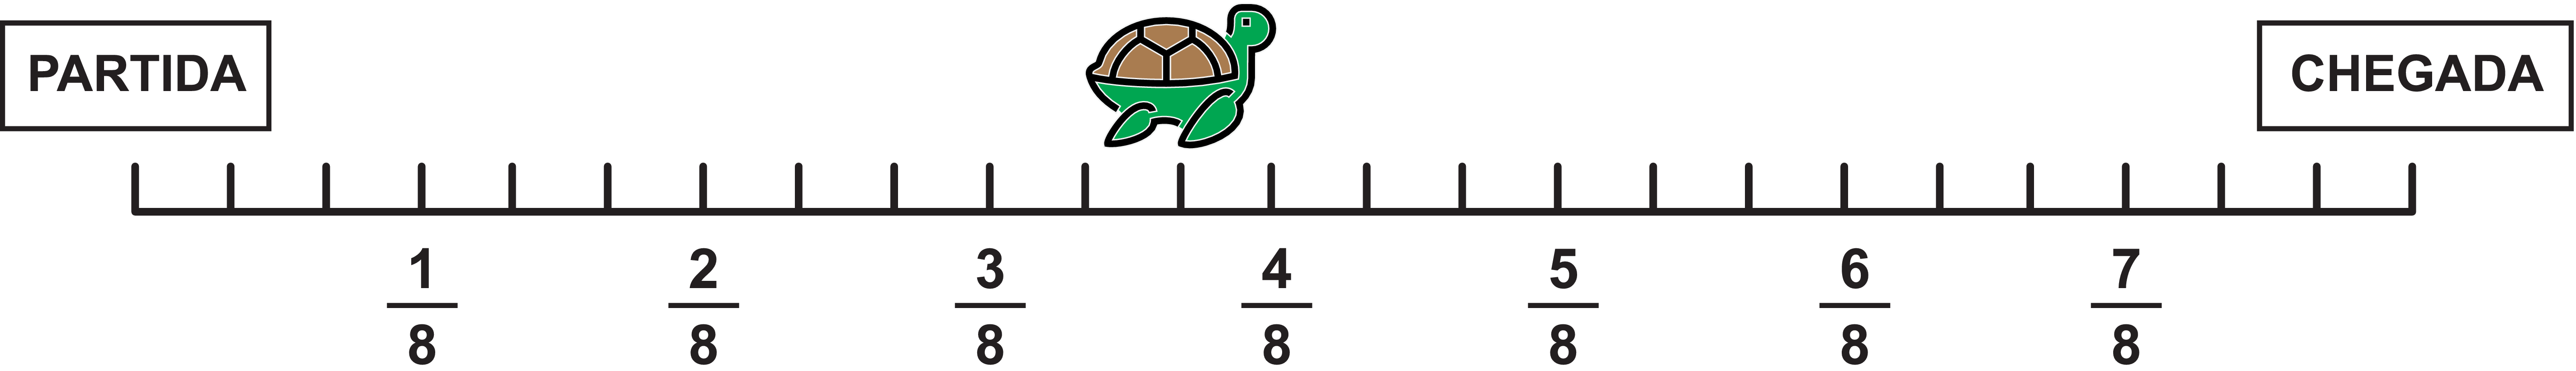
\includegraphics[width=390pt, keepaspectratio]{ativ9_resp_h}
\end{center}

\item     Está correta. De acordo com a resposta do item a), a tartaruga não alcançou a metade do percurso. Portanto, para alcançar a chegada, a tartaruga ainda precisa percorrer mais do que a metade do caminho.

\item     Não está correta. A tartaruga já percorreu mais do que      $\frac{1}{3}$     do percurso e todo o percurso corresponde a      $\frac{3}{3}$. Portanto, para alcançar a chegada, a tartaruga precisa percorrer menos do que     $\frac{2}{3}$     do caminho.
\end{enumerate}

\end{solucao}
\fi

\end{document}